\documentclass{acm_proc_article-sp}
\usepackage{fontspec}
\usepackage{xunicode}
\usepackage{amsmath}
\usepackage{graphicx}
\date{}
\newtheorem{lemma}{Lemma}


\begin{document}

\title{Implementing deep hypertext with embedded version control}

\author{Victor Grishchenko \\ \small Delft University of Technology, Ural State University }

\maketitle

\begin{abstract}
While text versioning was definitely a part of the original
hypertext concept~\cite{xanadu,hyp-ed-sys}, it is rarely considered
in this context today.
Still, we know that revision control underlies the most exciting
social co-authoring projects of today's Internet, namely the
Wikipedia and the Linux kernel. With an intention to adapt the
advanced revision control technologies and practices to the
conditions of the Open Web, the paper reconsiders some obsolete
assumptions and develops a new versioned text format perfectly
processible with standard regular expressions (PCRE~\cite{pcre}).

The resulting \emph{deep} hypertext model extends the linking
concept from inter-document associations to intra-document
dependencies and evolution. As the most promising consequence,
it allows decentralized real-time revision control in the Open
Web, i.e. co-evolution and mutation exchange among multiple
competing copies of the same text. 

\end{abstract}


\section{Rationale}

Historically, the object model of the World Wide Web is a graph
of pages connected by unidirectional links. In this context,
the value of a link is an association between two pages, while
evolution of a single page is out of scope and is more of an
obstacle as it potentially breaks links.
Such a Web may scale indefinitely; that cannot be said about
our perception. So, normally we resort to a search engine to rank
all the pages and to return those most relevant to us.
During the last decade, we have also witnessed the fundamentally
different \emph{wiki} approach of synthesis, the most notable
example being Wikipedia, when a multitude of contributions is
fused into a singular document which an end user is able to consume.
This process of knowledge fusion is inherently social and
focuses on the evolution of a single document.
Naturally, that process is based on revision control technologies,
and it should be noted that Wikipedia's version control
technology is as obsolete as you can possibly get, especially
if compared to the recent developments in Source Code Management
(SCM) employed e.g. by Linux kernel developers or other 
large-scale software development projects.
At a smaller time/size scale, document evolution and revision control
enable group collaboration environments, notable examples
being Etherpad, Google Docs, Google Wave.

Given the potential of the knowledge fusion process, the idea
of adapting advanced revision control technology to the conditions
of the Open Web naturally comes to mind (``open'' both in the
sense of open sea and open standard). 
Indeed, all the advanced SCM techniques, such as branching,
3-way merging, distributed version control, et cetera, were not
introduced for the art's sake. Each technique has a purpose of
overcoming a certain scalability barrier that have emerged once
software projects became sufficiently big. 
Consider Wikipedia; it is certainly big and it certainly faces
a scalability barrier \cite{wp-elites, wp-decay}. In case
scalability issues are resolved, we
may witness something much more exciting and useful, maybe even 
a Web-scale Wikipedia housing both general and specialized
knowledge.

To give an introduction to the technical part of the problem we spend
Section~\ref{sec:scm} to
review the technological foundations of
revision control. As it was said, Wikipedia's technology 
is lagging 20 to 30 years behind the state of the art in the
source code management (SCM) field. 
In Section~\ref{sec:textile}, we proceed to the focal topic of
this paper which is
adaptation of advanced version control technologies for Open-Web
hypertext versioning. As a result, we come up with a vision of
\emph{deeper} hypertext carrying its history, authorship
attribution and internal dependencies.
Then, in Section \ref{sec:algos}, the concept is proven to be
practical by implementing both
basic and advanced revision control operations, mostly relying
on Perl-compatible regular expressions, which are readily available not
only in numerous programming languages, but even in the
constrained environment of a Web browser, thanks to JavaScript.
The concluding Section \ref{sec:conc} hints at some promising
implications and consequences of the introduced technology.




\section{Revision control} \label{sec:scm}

Just to give some introduction, I will first outline some current
trends and tradeoffs of revision control. The most
basic decision and tradeoff of a revision control system
is the versioned data
storage format. The simplest form of storage format is \emph{snapshots}:
every next version is just dumped to the storage. The simplistic
approach has a serious shortcoming: the space consumed by the storage
tends to grow as $O(N^2)$, where $N$ is the size of the file.
That is caused by the fact that every small change causes the
entire file being written all over again. In particular, Enlish
Wikipedia (enwiki) clearly faced that problem; their last successful
full-history dump was made on January 2008. Smaller pedias are
still doing quite well; apparently their $O(N^2)$ is not
out of bounds yet.
As an extreme example, snapshot storage is totally
unacceptable for real-time version control, where changes
are introduced symbol by symbol, so the $O(N^2)$ would be quite
close to exactly $N^2$ of storage ($10^{6}$ for 1KB of text,
$10^{8}$ for 10KB etc).

An improvement over snapshots is \emph{delta}-based storage. 
Delta storage keeps just some versions of a file as snaphots,
the rest being stored as a sequence of deltas. To recover a
historical version, a number of deltas should be applied
to a snapshot. 
So far, this method is the most popular among revision control
systems. The git~\cite{git}, for example, formally employs
snaphot storage, but older revisions are delta-compressed
for storage efficiency. 

The third classic storage format is the 
\emph{weave}~\cite{rcs-txt,revctrl-weave}. 
A weave contains all the pieces of a text that ever existed,
in their natural order, annotated with their birth and
death ``dates''. Given a certain revision id, a weave may be
scanned and all pieces alive at that point in time will form the
corresponding version of the text. Weave is traditionally
considered complex to implement, it also suffers of high 
input-output overhead~\cite{bazaar-weave} as the entire
weave has to be overwritten on every change. As a consequence, 
it is not widely used as a storage format.
An attempt to adapt the classic weave format for non-linear
history seemingly makes it even more complex.

Meanwhile, mass migration to non-linear development and distributed
version control systems is the most notable trend of past
years. Linux is developed with the git, Google Code adopted
Mercurial~\cite{mercurial}, and numerous open source projects head in the
same direction, migrating from legacy CVS or Subversion.
The advantage of distributed revision control system (RCS) is the ability
to routinely support numerous semi-independent versions
of a project which fork and merge back.
Fundamentally, it allows for better scalability of
software development: more people doing more things at
once without causing chaos.

Another promising trend is the emergene of real-time
revision control systems, mostly used in groupware.
An earlier example, the Google Docs, recycled the classic revision
control techniques~\cite{diff-match-patch}, such as
patches~\cite{patch} and Meyer's diff~\cite{meyer-diff};
it just invoked those operations more often, automatically.
The recent Google's project Wave adopted true
real-time approach derived from the previous academic
work on Operational Transformation (OT).
OT starts at the same positions as the classical revision
control techniques: a text is a chain of atoms,
any changes are represented as insert or remove
\emph{operations} at certain positions in the
text. The problem is, once editing is done concurrently,
those operations cannot be integrated easily. The position
numbering depends on previous changes and once some previous
changes are concurrent and thus unknown, position numbers
become inconsistent. The classic diff-match-patch approach
employs a set of heuristics and combinatorial algorithms
to apply changes properly; position numbers are always
considered as approximate, every change is shipped with
its \emph{context}, i.e. chunks of unchanged text before
and after the changed area.
The OT approach instead applies
\emph{transformations} to the mutation operations to amend
the position numbers and to integrate concurrent
changes consistently. The OT theory~\cite{sun-achieving} mentions
three basic consistency requirements, also known as the CCI
model: 
\begin{itemize}
\item causally dependent operations are always
executed in their cause-effect order (causality)
\item all sites converge to the same state of text once
they execute the same set of operations, independently of
their order of arrival, which may vary due to concurrency (convergence)
\item the effect of executing an operation is
always the originally intended effect; position shifts must
not cause misapplication of operations (intention preservation)
\end{itemize}
The only problem of OT theory is, informally, its legendary
complexity, approaching that of the string theory.
Very similarly, there are numerous classes of OT flavours\cite{ot}.
It should be noted, that at least the Wave's OT flavour
is centralized as it needs a single
central authority to order concurrent changes in a single
consistent way.

At this point, it makes sense to reconsider two basic
assumptions of the classic revision control, as they seem weak
in the present circumstances. First of all, that symbols are
necessarily
addressed by their positions in a text. The method introduces
numerous unpleasant consequences, as position numbers
in a changing text are less than unreliable. 
Assigning unique identifiers to symbols was historically
considered to be too complex or too expensive.
Second classic assumption to be questioned is the
separation of a revision control program from an
editor program, so the former only accesses some snapshots
of the text made by the latter.
The revision control program is supposed to
run the longest common subsequence algorithm~\cite{lcs-algo} to
recover what actually happened to the text.
This unfortunate loss of knowledge inbetween two
applications is avoided in the
case of Web-based real-time editing applications, where
every keystroke made by the user is instantly known.
It is likely to be avoidable in many other cases;
e.g. once revision control code is easily embeddable.


\section {Adaptation}   \label{sec:textile}

Back to the objective of adapting advanced version
control technology to the Open Web, let's consider the
requirements and the corresponding problems of the
current technologies. Once the problems are listed, I
will outline the proposed solution.

\subsection {Problems}
First of all, revision control is normally implemented
in complex standalone software. Although there are JavaScript
implementations of basic algorithms such as Fraser's
diff-match-patch~\cite{diff-match-patch}, those are
heavyweight heuristic-rich combinatorial
algorithms and, frankly, better be optimized out
completely. We will target a set of version control
algorithms entirely implementable in 
linear-complexity regular
expressions without any combinatorial part.

Second, both to exclude position-dependent logic and
to allow for truly real-time revision control, we will
represent all mutations at single-symbol granularity,
each symbol being uniquely identified. Such uniquely
identified symbols are named \emph{atoms}.

Third, the problem of merging concurrent changes must
be resolved in a simple automatic way, without any user
intervention. It should be noted, that
\emph{semantically} correct merge of changes is impossible
in principle: semantically correct concurrent
changes, being merged cleanly in
the technical sense, still may produce a semantically
incorrect result and there are no way to prevent that
from happening,
apart from employing some sort of artificial
intilligence. Thus, real-world RCSes focus on technically
correct merge, resorting to human intervention in case
some heuristics detect a dangerous situation (e.g.
concurrent changes to the same line).
We will focus on technically correct and predictable way
of merging, additionally emphasizing the convergence
requirement.

Fourth, versioned data formats tend to be quite
complex. We will use only string-based formats,
composed of equal-width fields; those are effectively arrays.
Both strings and regular expressions belong to the standard
toolkit of any high-level language (except probably
Erlang); they are highly-optimized and work at nearly-native
speeds at worst; in some browsers~\cite{wrec}, regexes are
directly compiled into machine code.

\subsection{Data structures}

Our basic data structure will be a \emph{yarn}, a sequence of
symbols introduced to a single page by a single author.
A yarn is identified by its URL.
Every symbol in a yarn is identified with its offset,
but instead of numbers we will use single Unicode code points.
A yarn may reference other yarns, in case the page was
co-authored by multiple authors.
Thus there exists \emph{frame}, an append-only list
of referenced peer yarn URLs. Each peer yarn is thus
identified by its offset in the frame list, also represented as
a single Unicode codepoint. A full identifier of an atom
consists of two chars: one char for its yarn, another
for its offset within the yarn. This in turn creates
different forms of atom encoding, such as 1-form
(the symbol itself) or 3-form (a symbol and its full
identifier).
Further on, data structure names will be postfixed
with the width of the form they use, e.g. {\tt yarn3}.

The second basic data structure is a \emph{weft}, which
is effectively a revision's identifier. A {\tt weft2} consists
of (yarn id; last symbol id) pairs, and points at the
revision when those yarns were that long. 
In some sense, a weft is drawn across the yarns,
hence the name. A closed weft is
a weft unchanged by transitive closure, i.e. inclusion of
all the recursive dependencies caused by yarn-to-yarn
references. The {\tt weft1} format is more condensed:
it only includes last symbol ids, sorted
according to alphanumeric ordering of their yarn URLs.
%As the yarn list may extend over time (new authors join), the particular subset of mentioned yarns is defined by the length of {\tt weft1}.
Wefts are essentially vector clocks,
see Sec.~\ref{sec:lamport}.

Single symbols are linked into a text through the causality
relation. A symbol is said to be \emph{caused} by its preceding
symbol at the time of
insertion. This adds three other forms: 5-form (the symbol, the causing
symbol's id, own symbol's id), 3c-form (the symbol and the causing
id) and 5c-form (the same as 5-form, but the causing atom id
goes first).

\newcommand{\aum}{{\fontspec{Devanagari MT}\selectfont ॐ}}
\newcommand{\eoa}{{\fontspec{Geeza Pro}\selectfont ۝}}
\newcommand{\bsp}{{\fontspec{Apple Symbols} ⌫}}
\newcommand{\zero}{{\fontspec{Apple Symbols} ⌀}}
The causality relation forms a tree of atoms.
To give that tree a simpler single-root form we define zero
state of any text to consist of two special symbols: start (the root)
and end, designated as \aum ~and \eoa. Any actual symbols are
inbetween those two.
In case a text was uninterruptedly typed, its causal tree
degenerates into a mostly-chain, except for the \eoa ~symbol.
In either case, depth-first preorder traversal of the tree
produces the text. A closed weft cuts a rooted subtree out
of the whole tree; that subtree represents a revision.
A causal tree grows in a very natural way, by forking and
growing branches.

The third basic data structure we use is the weave, 
normally {\tt weave5c},
which consists of all the symbols that ever existed, in order. 
Deleted atoms are followed by backspace atoms \bsp; backspaces
are normal atoms in most regards.
Past or present revisions of a text are derived from its
weave given a weft.
All modifications and transformations of a weave are done by
regular expressions, while those regular expressions are often
produced by other regular expressions. The intricate dynamics of
the process is considered in greater detail in the 
Section~\ref{sec:algos}.

\subsection {Sibling ordering}  \label{sec:siblord}

It should be noted that causality is a partial order, so it
cannot directly order atoms totally into a text. Namely, it
omits ordering of siblings; in case two symbols were inserted
after the same parent symbol, their causal order is undefined.
For example, the first symbol of the text is a child to \aum
~and a sibling to \eoa. We will define a specialization of  
the causal ordering to resolve the issue.

An atom $a$ is \emph{aware} of atom $b$ if $a$ is caused
by $b$ or $a$ appears later in the same yarn as $b$ or
there is a chain of those two relations connecting $a$ to 
$b$ through some intermediary atoms.
Informally, awareness means that at the time of insertion
the author of $a$ knew $b$ existed. For a given atom, all
atoms it is aware of form a subtree that may be described
by a weft.
The awareness relation is reflexive, asymmetric, transitive TODO.

The awareness order is 
defined as a preorder depth-first traversal of the causal
tree, where aware (i.e. yonger) siblings are traversed first,
%once $a$ is caused by $b$, $a$ is certainly aware of $b$,
e.g. the first symbol of the text goes
before \eoa. In many cases, awareness should be manifested
manually. Namely, once an author is inserting symbol $a$ after
a symbol $b$ that already has a child $c$, and awareness
cannot be derived from the existing context, then the author is
supposed to first insert a fictive zero-symbol \zero ~after $c$
to signal awareness.
Zero symbols are included into the
weave, but are never shown in the resulting text; the same
applies to other special symbols: \aum, \eoa, \bsp.

The resulting ordering is still partial, as the authors
may be unaware of each other doing concurrent changes, so
the awareness relation still might be undefined for some
siblings. Thus, we finally introduce the total order
which, be it introduced earlier, might have caused confusion.
The \emph{weft order} assumes that all atoms are ordered in
accordance with depth-first preorder traversal of the causal
tree, while siblings are traversed in the descending 
alphanumeric order of their awareness {\tt weft1}.
This is a specialization of the awareness order, because
awareness is transitive and, correspondingly, if $a$ is
aware of $b$, then $\tt weft1(a) > weft1(b)$. The inequality is
strict because two symbols cannot be aware of each other
(circular dependency), so their wefts surely differ.

While weft lengths may grow with the time as more authors
join, the relative order of two {\tt weft1}s never flips.
Assuming that we compared those two wefts at a moment when
their lengths were $l$, then arrival of additional $k$ coauthors
will extend those wefts to the size of $l+k$ symbols. Still,
the extension is done by inserting zero symbols at exactly
the same positions, corresponding to the positions of URLs
of the newcomer authors in an alphabetically sorted list
of yarn URLs. As all newcomer positions in both wefts have
equal zero values, they are irrelevant for ordering.

The described formal system is based on simple definitions
and, in most cases, it is easily implementable with regular
expressions. For example, an operation of removing every
symbol followed by a backspace is just trivial. That cannot
be said about the ordering of unaware siblings; they are
truly hard to implement in regular expressions. While the
situation of two symbols concurrently inserted at the same position
in the text might not be that typical, it is still critical
to hold the convergence requirement without any resort to
central coordinating entities. Namely, that all distributed
replicas of a text must converge to the same state, if
supplied with the same set of changes (atoms), independently
of the order of arrival.

To ease implementation of that tricky case, I will prove
a small lemma. It will also shed some light on the
correspondence between the causal order and the order of atoms
in a weave.
First of all, a causal subtree rooted at some atom occupies
a solid interval in the weave; that is just a feature of
depth-first traversal. Let's call it a causal block.
A causal block starts with its root atom; the rest is
a sequence of zero or more causal blocks of its children.
The question is: how will we locate the end of a causality
block?
\begin{lemma} A causal block rooted at $r \ne$ \aum ~lasts till
the first atom $b$, whose parent is not $r$ but an atom
$r$ is aware of (exclusively):  $cblock(r) = [r,b)$. 
\end{lemma} \label{lemma:1}
Proof. $b$ is the first element to the right from the causal
block of $r$; $b$ surely exists. Parent of $b$ is an atom $p$,
which resides in the weave somewhere to the left from $b$.
$p \notin [r,b)$, because otherwise $b$ would also belong
to the causal block of $r$, contradiction.
Then, $p$ is to the left from $r$. Consequently, $r$ belongs
to the causal block of $p$, $r \in cblock(p)$, because
causal blocks are solid intervals and both $p$ and $b$
belong to $cblock(p)$. All atoms within a causal block are
immediately or transitively caused by its root,
ergo $r$ is aware of $p$. At the same time, no atom
within $cblock(r)$ has a parent $r$ is aware of, unless
that parent is $r$, because $r$ cannot be aware of the
atoms it caused. Proven.

\section{Implementation}	   \label{sec:algos}

\begin{figure} \label{fig:ops}
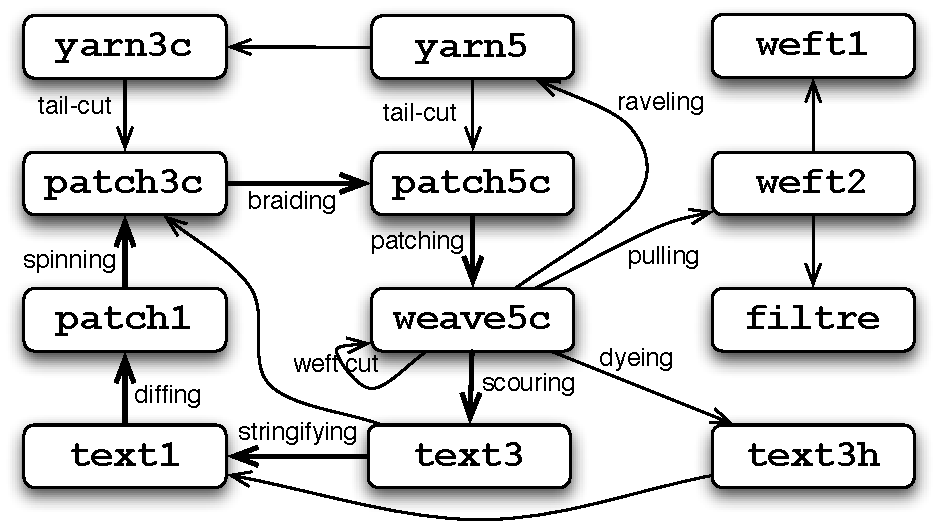
\includegraphics[width=0.48\textwidth]{operations.pdf}
\caption{Causal model formats, operations and dependencies.}
\end{figure}

As the number of formats and operations employed in the
causal tree model is quite high, see Fig.~\ref{fig:ops}
for a general overview.
For easier narration, this section will describe a
typical workflow loosely based on the scenario of 
collaborative text authoring by several users connected
to a single server. Key regular expressions will be
mentioned, using a Perl-like notation.

The central format of the model is {\tt weave5c}, a weave
where each atom is represented by its symbol, then
two-codepoint id of the causing atom, then two-codepoint
id of the atom itself, five codepoints total.
Weave might be transformed into {\tt text3} by 
\emph{scouring}: removing all the deleted atoms and all
the special symbols from the weave: \\
{\small \verb`s/(...(..))(\b\2..)+|[\b].{4}|.\0.\0.|(.)..(..)/$4$5/g`}
The expression filters out any symbols that were deleted
i.e. those that caused (are immediately followed by) an
\bsp ~atom.
Out of the atom's 5-form, only the symbol and its id are
taken, thus the output is a 3-form. {\tt text3} might be
trivially stringified into {\tt text1}, i.e. the text
itself: {\small \verb`s/(.)../$1/g`}.

The text is then put into the editor; a user makes some
changes. Those changes might be tracked either by listening to 
basic events or by comparing text snapshots with 
any flavor of the diff algorithm or heuristics.
The result is a chain of {\tt patch1} substrings
corresponding to inserted and removed portions of the text;
their offsets at the original text are known. That allows
to check {\tt text3} for atom ids corresponding to the
change: wither attach points for insertions or sets of
removed ids for deletions. That allows to spin {\tt patch3}
and further 
 to braid a {\tt patch5c}, which contains all
the inserted atoms in the 5-form. 
{\tt patch5c} should be distributed to other users;
once it arrives it is ready to be integrated into the weave.
First, it is split into causal blocks; one block is typically
a causal chain of atoms corresponding
to a period of uninterrupted typing.
A block has a single attachment point
in the causal tree and might be inserted into the weave as
a substring.
Its insertion point is just after the causing
atom of the block's root atom, unless there are unaware
siblings. The case of unaware siblings will be considered later;
as a safeguard we just check that the root atom
is aware of the current right neighbor of its causing atom: \\
{\small \verb`s/^((?:.{5})*?)(...$C([\b\7\0]$C..)*)(?=...($F))/$1$2$P/`}\\
This regex clearly needs explanation. First of all, the regex
is anchored to the beginning of the string to ensure it
always matches with $\times 5$ offset and never across 5-form's atom
boundaries. Second, the regex is
composed using three variables: \verb+$C, $F, $P+. \verb+$C+
is the atom id of the root's causing atom; \verb+$P+ is the
{\tt patch5} itself; \verb+$F+ is an awareness {\tt filtre}
of the root atom. Filtre stands for ``filtering regular
exppression''; {\tt filtres} are produced from {\tt weft2} by
another regex, e.g. {\tt filtre('a2b4') = 'a[0-2]|b[0-4]'}.
A {\tt filtre} matches two-codepoint atom ids that fall within
the causal subtree cut by the {\tt weft2}. Another common
use for {\tt filtre} is to obtain a historical revision of a
weave: 
{\small \verb`s/(...($F))|.{5}/$1/g`}, which in turn
may be scoured to get a historical revision of the text.
In the case of patching, we produce a {\tt filtre} out of
the root symbol's awareness {\tt weft2} to ensure the author
of the head symbol was aware of the symbol to the right 
(no unaware siblings).

Well, what if there are unaware siblings, possibly introduced
by other users, so the first method of patching fails?
This is exactly the situation to apply the Lemma~\ref{lemma:1}. 
We single out the causality block of
the roots's causing symbol, then we split it into causality
blocks of the root's siblings, then we insert our block between
its sibling causality blocks,
according to the {\tt weft1} ordering (see Sec.~\ref{sec:siblord}).
The implementation of this case is quite complicated. While
still relying on on regular expressions, it involves some
non-trivial logic and, most importantly, the costly operation
of \emph{pulling} (awareness weft derivation), which does
several passes of the weave.
The assumption is that concurrent
insertion of symbols at the same position in the text is
a rare event, so this non-trivial machinery will be rarely
invoked.
It should be noted that the no-unaware-siblings patching case
employs awareness wefts as well. Luckily, in that case
wefts might be cached and incrementally updated
due to append-only nature of yarns, so the costly recalculation
is unnecessary.

So, we went through the full cycle: from a weave to a text
to a patch and back to the weave. Other operations are less
critical for the understanding of the model. For example, the
operation of \emph{dyeing} derives a {\tt hili3}, which is a
``painted'' text in a special 3-form showing the difference
between two revisions of a text. Namely, instead of the standard
(yarn id; symbol id) pair, a symbol is followed by a pair
of yarn ids: one for a yarn that inserted that atom,
another for a yarn that removed that atom. If no such
change happened between the two revisions, then id is null.
The {\tt hili3} string may then be transformed into
highlighted text or HTML.

Due to space constraints,
I will omit algorithms of dyeing and  pulling and the specifics
of processing deletions and undeletions in bulk.

To summarize, the model now implements all the basic
functions of a revision control system in a simple, 
portable and truly decentralized way.

\section{Estimations}

Let's consider practical feasibility of the introduced model.
I will consider issues in the ascending order of their
importance. First, all the operations
listed in the previous section run in negligible time
even on bigger texts. If ran within a browser, $O(N)$
regular expression passes a 1MB string in around a millisecond.
The patching operation for the case of unaware siblings may
take more time, let it be 100ms, but it is supposed to be a rare
``once a year'' case.
Second, while the overall computational cost of assembling a weave
from source yarns is $O(N^{2})$, i.e. a combinatory
explosion is possible, unless the weave is cached. In the
latter case, $O(N^{2})$ accumulates historically, over the
years of the text's lifetime. 
Third, using Unicode codepoints as, essentially, numbers
might seem risky. In fact, common regular expression engines
reliably support only the first 50,000 codepoints or, more
precisely, the $[U+0,U+D800)$ interval. In case an author
types in more than 50K of symbols, he should be assigned
another yarn id. In total, the capacity of this numbering
system limits text size to $2,5\times10^9$ symbols, which is more
than enough (three volumes of ``War and Peace'' in Russian
take 2,56MB in UTF-8). 
The 50,000 codepoints limitation also limits the number of yarns
and, correspondingly, coauthors of a single document
Practically, it is hardly a problem, as even the most popular
project, namely Wikipedia, has only three articles with an author
count above $2^{15}$: the Introduction, the Sandbox and the
Archive of the Sandbox, i.e. pages every new user predictably
bumps into. Excluding the exercise, complaint and similar pages,
the topmost ``real'' page has an author count of 13680 as of
the 2009-08-16 snapshot. That is the ``George W. Bush'' article
and the reasons for the high author count are likely to be
similar to the Sandbox case.


The size of a text or a weave is not of big concern as well,
as texts are small in general: Web traffic 
is dominated by images, not to mention video content.
Weave actually holds the entire text's history, so it may
be substantially bigger. But for practical everyday use,
full weaves are
not necessary, as the user is more likely to be interested
in the changes since the last visit, not the full mutation
history. Thus, some distilled version of a weave may be
used, long-dead parts being {\tt filtre}d out. Another general
consideration is that the amount of processed information
(think of the Web) tends to grow exponentially and, due to
$\int e^{cx}dx = \frac{1}{c} e^{cx}$, the mass of the last
revision is likely to differ from the mass of the full
history (i.e. weave) just by some factor. As the saying
goes, ``devil is in the details'', so let's consider the
actual numbers.

\begin{figure} \label{fig:weave}
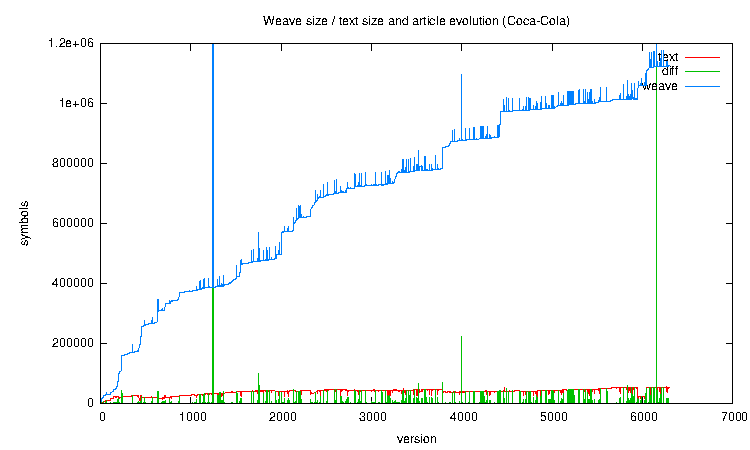
\includegraphics[width=0.48\textwidth]{cocacola-weave_vs_text-linscale.pdf}
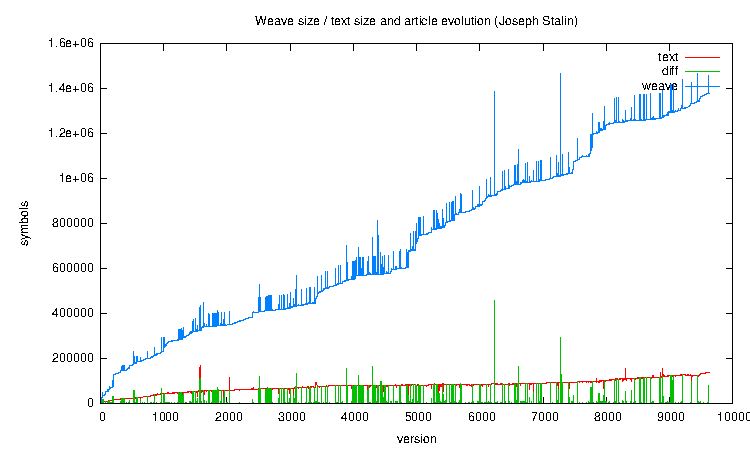
\includegraphics[width=0.48\textwidth]{stalin-weave_vs_text-linscale.pdf}
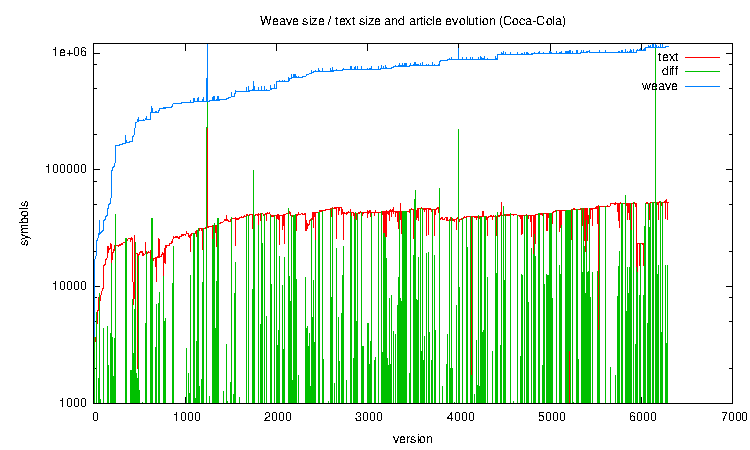
\includegraphics[width=0.24\textwidth]{cocacola-weave_vs_text-logscale.pdf}
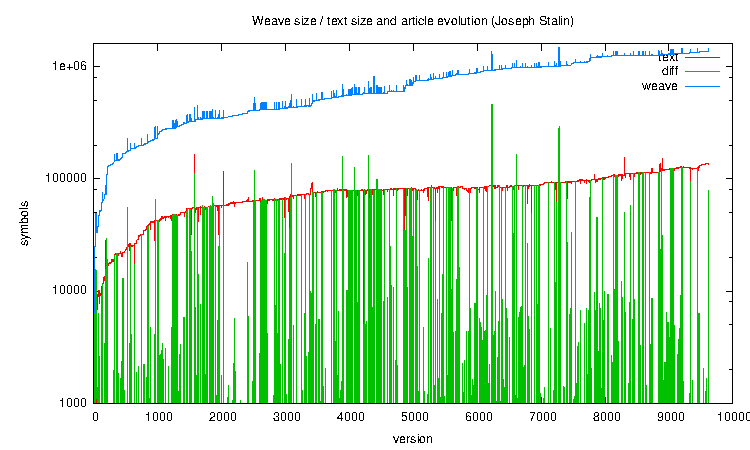
\includegraphics[width=0.24\textwidth]{stalin-weave_vs_text-logscale.pdf}
\caption{Weave size evolution experiments. Top: text, diff and weave sizes for the ``Coca-Cola'' and ``Joseph Stalin'' articles. Bottom: same graphs in log-lin scale (sizes are logarithmic).}
\end{figure}
To estimate growth dynamics of a weave, I plotted
weave size evolution for two popular Wikipedia pages: ``Coca-Cola''
and ``Joseph Stalin''. Weaves were derived form the full
history dump dated January 2008 (the last successful one
for enwiki). The results are shown at Fig.~\ref{fig:weave}.
Vandalism was intentionally filtered out as it specifically
inflates size of a weave (the entire text is deleted, then
recovered back). Namely, all changes that were rolled back
within 20 revisions were not counted; I was checking for
pairs of identical revisions to declare a rollback, so
some vandalism acts were left undetected; still, that simple
criteria provided a clear enough general picture.
Roughly, weave size grows linearly with the number of edits,
as well as the article size, except an article is sometimes
gets rafactored and shrinks. As a rule of a thumb, \emph{full} weave
size may be estimated as x50-x100 the plain text size.
Mass of a prefiltered weave is likely be around
text size times 5 or 10, depending on charset/encoding,
which factor is defined by the form-5 overhead.

Interestingly enough, a gzip of
snapshots is far worse than an uncompressed weave (see
Fig.~\ref{fig:sizes}). A
7zip archive is better off, its main shortcoming being high CPU
consumption (it took 20 seconds to unpack one of the articles).
As a summary, weave is effective as a server-side versioned
text format. For the client side, a weave better be prefiltered
to keep only those changes of interest.


\begin{figure} \label{tab:sizes}
\begin{tabular}{|c|c|c|}
\hline
Article & Format & size \\
\hline
Coca-Cola & plain snapshots & 253,760,722b \\
Coca-Cola & .gz of snapshots & 78,450,167b \\
Coca-Cola & .7z of snapshots & 481,952b \\
Coca-Cola & weave5c & 1,126,011c \\
Coca-Cola & text1 & 52,477c \\
Joseph Stalin & plain snapshots & 753,906,073b \\
Joseph Stalin & .gz of snapshots & 281,409,652b \\
Joseph Stalin & .7z of snapshots & 891,514b\\
Joseph Stalin & weave5c & 1,379,858c \\
Joseph Stalin & text1 & 137,088c \\
\hline
\end{tabular}
\caption{Space consumed by history storage in misc formats; postfix ``b'' stands for bytes, ``c'' for Unicode chars (byte size may vary depending on charset and encoding).}
\end{figure}

Finally, as we talk about data storage formats, it is
definitely useful to consider their IO patterns. A weave
is convenient for reading and processing, which is done in
sequential passes. It is much less convenient for writing,
as it needs to be overwritten entirely after any
modification. A yarn is exactly the opposite: it is
append-only, so writing is cheap, while reading and
weaving together many yarns is both cycle and IO
consuming operation.
In practical scenarios, mixed solutions are better.
As an example, consider the {\tt weave5c+patch5c+text1} set.
Read-only clients may be served with {\tt text1}. All
ongoing modifications might be appended to {\tt patch5c},
which thus acts as a write cache. The {\tt weave5c}, once
read from the disk, should be immediately  updated with
the {\tt patch5c}. Once {\tt patch5c} becomes too
big, the weave might be overwritten with its current
version, {\tt patch5c} is thus emptied. Other mixes are
also possible, depending on trade-offs. For native (non-regex)
implementations, tradeoffs might be different; e.g.
a {\tt weave5} might be assembled from {\tt yarn3c}s
in linear time; as yarns are append-only they are also
perfectly cacheable, etc etc.

Note. Order of atoms in a weave does not depend on the order
of their arrival. Total order. Correctness.
By design: no violation of awareness, dfs order.

\subsection{Sectioned model}

The causal trees model exclusively considers plain/flat text;
formatted text is often modeled as a tree structure, e.g.
HTML's Document Object Model (DOM)~\cite{dom}. I will sketchily
address this concern.~\footnote{My understanding of what should
and what should not be done here is based on the experience of
building a chain of prototypes over the past 
years~\cite{www06,csr07,wikisym08}.} 

While DOM imposes hierarchical structure on formatted text,
the text per se was not historically considered hierarchical,
except probably for its bigger units, i.e. \emph{sections}. 
Consider LaTeX, the RFC text or the wikitext format or even the
early pre-DOM HTML: the text is considered to be a flow of
words and markup elements, the only hierarchically structured
parts are sections/subsections. As a matter of fact, browsers
start with the ``tag soup'' model, later applying some
heuristics to transform it into an orderly tree. 

Note the open possibility to handle units of text hierarchical
structure (sections) separately. While each section might
be considered flat in the pre-DOM HTML sense, different sections
might reference each other through transclusion links thus
forming a hierarchical structure. Each section has its own weave;
as a weave is just a string, the resulting data structure is
simple enough.
As a result, we have a digraph of sections;  
that keeps the complexities of the document's hierarchy and
revision control orthogonal.

Of course, in the context of HTML, correct XHTML structure cannot
be guaranteed when merging concurrent modifications: for example,
two overlapping tag ranges cannot be merged correctly in the
general case, e.g. \verb+<i>Quick <b>brown</i> fox</b>+.
That of course returns us to the tag soup situation; but that is
the state of the things anyway and  browsers are good in dealing
with it. In either case, this alternative seems more practical
than distributed real-time revision control of DOM trees
(see Sec.~\ref{sec:waveot}).


\section{Parallels and reflections}

Throughout the paper, our model was compared to the classic
diff/patch/snapshot revision control paradigm. It certainly makes
sense to put it in a broader context to uncover diverse
similarities and dependencies.

\subsection{Operational Transformation}

First of all, the causal model fulfills three requirements of OT.
Causality preservation holds
by design, as an atom is never introduced to the weave before all
any of the atoms it is aware of TODO.
Convergence is insured as the order of atoms in a weave does
not depend on the order of arrival (prove). Intention
preservation, in the sense of applying changes to a wrong position
in the text, is trivially solved: the logic is not positional.

Differently from operational transformation schemes, causal trees
absolutely lack the transformation aspect: atomic operations
stay intact and interact in simple predictable ways. That brings
it closer to the "European school" of operational transformation
that abandons positional logic in favor of unique atom
identification.

\subsection{Fidge-Lamport vector clocks} \label{sec:lamport}

The causal tree model perfectly matches entities of the
Lamport-Fidge vector/logical clocks model. Namely, yarn
corresponds to a process, foreign causality relations - to
messages, yarn offsets to local logical clocks and wefts to
vector clocks. Still, yarn offsets do not correspond to Lamport
timestamps, as there are no rule to synchronize them.
Awareness order follows the lines of Lamport's synchronized
logical timestamps. The weft order is similar to Fidge's vector
clock ordering, but there are no strict equivalence here.

\subsection{Xanadu}

There are some parallels between causal trees and the historical
Xanadu hypertext model. The spirit of Xanadu is to keep all the
versions of all texts at the same time, by clearly separating the
primary input from the actual revisions of the text. Very similar 
approach is seen in causal trees: primary input is put into yarns
while all the actual revisions are subsequences of the weave.

\subsection{Wikipedia}

Currently, Wikipedia faces scaling problems; nature of those
problems is quite complicated and cannot be discussed in this
article. Still, it is author's belief that TODO
A fork of Wikipedia might always be done, but the contributors
will stay with a single project and no content exchange between
two branches will be possible. That is in drastic contrast with
the state of things in source code version control; easy content
exchange between numerous branches is the very foundation of
distributed version control. That raises a question, whether it
is possible to introduce version control technology to allow
competition of multiple versions of Wikipedia, still maintaining
regular content exchange. A Web-ready revision control technology
might enable the scenario.

\subsection{Google Wave}  \label{sec:waveot}

Google Wave relied on a flavor of Operational Transformation for
real-time version control. The enhanced OT flavor is supposed to
handle both plain text and tree-like XML DOM structures.
Informally, the main problem of the resulting technology is that
its complexity is OT complexity \emph{times} XML complexity. 
The authors even had to enrich XML with additional entities 
named ``annotations'' to make it suitable for their needs.
There are 15 sorts of different mutation operations used in Weave
OT, some as opaque as ``delete anti-element end''~\cite{waveot}.
Theoretically, the potential for unexpected feature interactions
tends to grow combinatorially with the number of primitives.
In practice, the overcomplication resulted in numerous bugs and
slow, unresponsive user interface~\cite{own-experience}.
According to an insider~\cite{gerasimov}, in 6 months since the
projects's launch the possibility of working with partial
histories is not  implemented yet; pages are bootstrapped with
their complete histories. Compare that to the ease of applying
a filtre to a weave in the CT model.


\section {Conclusion}

While many previous revision control solutions were either
fully distributed or real-time or Web-based, the causal trees
combine all that at once. Thanks to a very simple string based
format and trivially portable regex-based algorithms, causal trees
have a good chance of making the critical step from an
application to a protocol used at mass scale in highly
distributed highly heterogeneous environment, i.e. the Open Web.


\section{2filter}

As it was mentioned, causality forms a tree, whose traversal
defines the weave. Still, causality is just a partial order
and the order of sibling atoms was not addressed. In case
several symbols were inserted into the 
Let's specialize the causality relation to incorporate sibling
ordering.
The ordering must always allow to insert an atom at a given
place and the relative order of atoms must not change over time
(no flips); that follows from the convergence requirement.
To define the order, we use the notion of awareness. 
   Informally, atom A is ``aware'' of B if a user who added A has
   also seen B. That might be the case if:
   \begin{itemize}
     \item A is caused by B
     \item A is in the same feed as B, at a latter position
     \item any chain of the above situations
   \end{itemize}




\begin{itemize}
\item version control system accesses the source occasionally (at the ``commit'' time)
\item the basic unit of change is a line of code
\item versions are synchronized via some central ``repository''
\end{itemize}
Recent trends reconsider those assumptions.
First, progress toward decentralized version control removed the notion of any central repository. Instead of a centrally-hosted tree of versions such systems as git~\cite{git} or Mercurial~\cite{mercurial} assume existence of numerous distributed and occasionally synchronized \emph{peer} repositories each containing a directed acyclic graph (DAG) of versions.
Second, real-time version control systems allow multiple persons to collaborate on a text in real-time. Real-timedness necessitates continuous access to the document as well as finer-grained change control;  symbols, not lines become basic units (``atoms'') of change.

Still, new efforts often focus on adopting the classical paradigm to new conditions. This article demonstrates that given the current conditions and tradeoffs, much simpler approach is feasible, effective and efficient.
Namely, that a real-time distributed version control system might be implemented in constraints of a simpler scripting language, such as JavaScript, leaving all the heavylifting to regular expressions and using JavaScript control and data structures as a glue.
The most intricate computational problems of classical version control  approaches, namely \emph{diff} and \emph{merge}, are trivially bruteforced. In particular, the change detection algorithm \emph{diff} becomes trivial as version control system might be instantly connected to the source code thus tracking every atomic change. Separation of the edits through combinatorial analysis of two snapshots using the longest common subsequence search~\cite{diff} now becomes unnecessary. The change \emph{merge} algorithm is bruteforced by (cheaply) assigning unique identifiers to all symbols of a text. Thus, detecting the insertion place by a mix of positional and contextual heuristics~\cite{fraser} also becomes unnecessary.

The presented model presents a fresh look on some classical tradeoffs of version control systems. Take, for example, the choice of snapshot-based vs delta-based vs weave-based storage. The presented model enhances the weave format to make its simplicity comparable to snapshots and its compression comparable to delta-based storage (See Sec.~??).


The paper makes heavy use of regular expressions. ``Regexes'' are adaptations of deterministic finite automata for text processing. This paper uses the popular perl-compatible dialect~\cite{pcre} of regular expressions also employed by the current generation of scripting languages (Perl, Python, JavaScript). Other constructs used, both control structures (ifs, loops, functions) and data structures (strings, integers, arrays, hash maps with string keys) are well-maintained in all mainstream scripting languages. Reliance on regular expressions allows to perform heavy operations with native performance -- this fact is critical, especially in the context of real-time version control.
Just to note the recent developments in regex performance, the WREC project (the WebKit Regular Expression Compiler~\cite{wrec}) managed to compile regexes directly into machine code thus achieving significant performance boost. Similar technique is employed by the Google's v8~\cite{v8-change-log}.

Regarding the adaptations of classical version control algorithms to the real-time case, the most notable current project is Google's diff-match-patch library~\cite{dmp} which powers Google Docs, recently Mozilla Bespin and other projects. Subjectively, d-m-p algorithms represent the case of ``a horseless carriage''. While being permanently attached to a webpage, they use combinatorial algorithms (Meyers' LCS~\cite{meyers}) when analyzing text snapshots to produce a patch. While being able to trace the origin of every single character, they use a fuzzy mix of positional and context-based heuristics~\cite{fraser-merge} to identify insertion points and deletion ranges on merge.

Another approach to real-time version control is Operational Transformation. It is a well-studied~\cite{ot1,ot2,ot3}, much less used real-time version control technology which is famous for its complexity and error-proneness~\cite{ot-mistakes}. The essence of the approach is to amend positional insert/remove operations to reflect the effect of other concurrent operations. The recently announced Google Wave~\cite{wave} technology's real-time editing feature is backed by a variation of Operational Transformation~\cite{waveot}. Complexity of the Wave's real-time version control might be informally estimated as complexity of OT \emph{times} complexity of extended XML (as of today, Wave employs custom extensions to XML~\cite{wavexml}). That is hardly satisfactory.

A notable branch of OT research is the ``European school'' of Operational Transformation~\cite{woot,inria,etc} which derived somewhat simplified methods for concurrent version control, mostly in the context of peer-to-peer/distributed wikis. One common feature of the approaches is the use of atom identifiers instead of positional addressing. While the text is composed of atoms, each atom mentions identifiers of its left and right adjacent atoms at the time of insertion, while algorithms focus on assembling the text to achieve the classic OT requirements of causality, convergence and intention preservation~\cite{ot}.

Regarding distributed version control systems, in recent years git~\cite{git} and Mercurial~\cite{mercurial} systems gained significant popularity; Codeville, Darcs and Monotone are less successful. Differently from the classical workflow centered around update/commit cycle, distributed version control systems focus on push/pull workflow for sending/receiving changes to/from certain branches of certain remote peer repositories. As a result, code changes traverse a ``social network'' of developers.


	
\section {Algorithms}

   Causal trees is a data structure devised for real-time distributed
   version control. As such, it is designed to process changes
   atomically symbol by symbol, to merge and branch versions of text
   trivially and unambiguously. The need for a new approach was
   dictated by the total inadequacy of the classical diff/patch model
   to the described usecase. In general, any positional version
   control scheme introduces lots of ambiguity when masses of changes
   are introduced concurrently and asynchronously in a totally
   decentralized environment. The notion of "position" in a text
   becomes extremely unreliable then. Thus, a step was made to
   uniquely address every single "atom" (i.e. symbol) in a "verse"
   (i.e. short version-controlled text). Even the data storage format,
   the "feed", was designed to allow separate storage and
   cross-referencing among text pieces introduced by different authors
   possibly residing in different administrative control domains. This
   section describes the basic versions of the relevant data
   structures as well as basic algorithms for processing them.
   
\subsection{Causality relation}   
   
   The specifics of the causal trees model are defined by its
   objectives of being a real-time distributed version control system.
   All changes are expressed in terms of atoms which correspond to
   individual Unicode symbols. The only relation among atoms is
   \emph{causality}: an atom is said to be caused by its immediate preceding
   atom at the time of insertion. For any given verse, the causality
   relation forms a tree of atoms, the causal tree.
   The root of the tree is the predefined atom named ``aum''.
   The linear form of the verse is defined by depth-first preorder
   traversal of the causal tree. The linear form is actually a weave,
   version control data structure containing all the pieces of the
   text that ever existed, in their natural order. The actual version
   of a text is derived by removing deleted symbols from the weave.
   Deletion is done by inserting a special ``backspace'' atom just
   after the atom to be deleted. 
   As atom addition is
   the only operation possible, atoms are stored and exchanged in
   feeds, append-only files containing atoms of the same verse, same
   author.
   
   As a rule, feeds, weaves and all basic data structures are stored
   and transmitted as UTF-8 strings to achieve both simplicity and
   minimal overhead even in higher-level languages. As well, most of
   CT model algorithms are implemented with regular expressions.

\subsection {The awareness relation}

   As it was mentioned, causality forms a tree, whose traversal
   defines the weave. Still, the order of siblings was not addressed.
   So, how atoms caused by the same parent atom are ordered? The
   ordering must fulfill two requirements:
   \begin{itemize}
     \item it must always be possible to insert an atom at a given place
     \item relative order of atoms must not change over time (no flips)
   \end{itemize}
   To define the order, we use the notion of awareness. 
   Informally, atom A is ``aware'' of B if a user who added A has
   also seen B. That might be the case if:
   \begin{itemize}
     \item A is caused by B
     \item A is in the same feed as B, at a latter position
     \item any chain of the above situations
   \end{itemize}
   Thus,
   sibling atoms are put in the awareness order: the text will read
   ``ABC'' if A is aware of
   B and B is aware of C (awareness is obviously transitive). 
   That would suffice
   is a synchonous environment given that any atom that has siblings
   somehow "declares" its awareness of them. For example,
   the late-comer atom might be preceded by a fictive
   {\textbackslash}u0000 atom caused by its sibling.
   Later, zero atoms are stripped from the text.
   In fact, such awareness-asserting fictive atoms let to use
   left-and-right-neighbor order, as it is the case with WOOT-related
   OT flavors~\cite{woot}. Still, that possibility is reserved for
   (rare) cases when it is actually necessary.
   
   Unfortunately, the awareness order does not suffice in asynchronous
   environments as sibling atoms might be introduced concurrently
   being unaware of each other. Thus, the awareness order is
   generalized to "awareness string order". An awareness string of an
   atom is a string composed of symbols of all the sibling atoms it is
   aware of, in their awareness string order plus the atom's own symbol.
   Effectively, an awareness string is a serialization of sibling
   awareness DAG (directed acyclic graph). In the causal tree,
   siblings are ordered in reverse alphabetic order of their awareness
   strings. Awareness strings do not change with the introduction of
   later atoms or addition of feeds; thus, no flipping of mutually
   unaware siblings is possible. Atoms whose awareness strings are
   equal, are considered to be the same atom.
   As an example, suppose siblings A and B are concurrently inserted
   after an atom O and later C is inserted just after O being aware of
   both A and B. Then, the resulting order is OCBA. The values of
   awareness strings are:
     A:    A,
     B:    B,
     C:    ABC.
   From the theoretic standpoint, awareness string order is essential,
   but practically any inconveniences caused by flipping of atoms are
   comparable to those caused by usual typos, being way less likely.
   For a single-server environment, it is just unneeded as any order
   introduced by the server is considered the right one. In
   Google Wave, for example, the ordering problem is resolved exactly
   this way: by ordering changes at a single ``authoritative'' server.
   Thus, a practical implementation may skip the awareness string part.
   
\subsection {Merging}
  Ideally, a merging algorithm has to integrate changes made concurrently
  by different authors to obtain a perfectly valid and meaningful
  document.
  It has to be noted that even valid and perfectly mergeable changes to
  distant parts of a text may ruin the text semantically. Even to a 
  greater extent that applies to code. Thus, semantic merging is
  impossible. Our objective is to merge changes in a predictable and
  technically consistent way.
  
  Precisely identified, flipping is impossible.
  Technical consistency, predictability,
   preservation of any contribution and resorting
  to manual semantical merge.
  
  Another important technical aspect is merging of HTML and, generally
  XML. In some cases, no generic merging solution exists. Consider the problem
   of two overlapping elements; say, a string ``\verb+text+'' being
  changed to \verb+t<i>ex</i>t+ by one user and to \verb+te<b>xt</b>+
  by another. Depending on the semantics of the tags,
  the results of a merge made by any given algorithm may vary from perfect
  to outrageous. As an example of a workaround for this particular
  issue, Google Wave OT extended XML with ``annotations'', a kind of XML
  ranges that may not abide the DOM tree  structure.
  Our approach is to keep things simple,
  treat a document as linear text and to leave markup
  merging issues to be resolved by different means.
  
   
\subsection {Lamport/Fidge model parallels}

At this point, it becomes clear that basic primitives of the CT model correspond well to primitives of the Lamport/Fidge logical clock model~\cite{lamport-clock,fidge-clock}, namely processes, events, messages and clocks. Namely, feeds correspond to Lamport's processes, atoms to events and causality relations to messages. The awareness relation perfectly corresponds to the Lamport's partial order $\to$. Correspondingly, CT sheds is another name for Fidge's vector clocks. While sheds are stored quite implicitly in the model, their use is a key to working with versions, see Sec.~\ref{sec:wl}.
%defining back cones and forward cones of events either affecting or affected by a given event. drawing inspiration from the relativity theory.
%This abstraction is essential for detecting dependencies, versions, assembly. E.g. a version of a verse is defined by a single atom is a single feed; the entire back cone is then a version. OT flavors were criticized for their use of vector clock. In the CT model, vector clocks correspond to awareness waterlines. Although they are not explicitly used or separately stored, they are easily derived.

\subsection {Practical algorithms}

A version control system contains two basic groups of operations: the ``workflow'' part and the ``history'' part. The workflow part has to implement \emph{diff}, i.e. detecting and serializing locally introduced changes and \emph{patch/merge}, i.e. introducing changes received from a remote party.
The history part involves all the operations for recovering historical versions and differences between them. The diff and merge problems are traditionally resolved using combinatory algorithms; in our case, the solution is obtained through brute force. As real-time version control tracks every user's action, detecting the difference is trivial. Merge does not pose a combinatorial problem as every atomic change has a precisely identified point of application.

Still, the absence of combinatorial algorihms does not imply total absence of algorithms. This section describes practical algorithms implementing all the key version control operations.
All data formats employed are Unicode strings; support of the Unicode Basic Multilingual Plane is implied~\cite{unicode}. All transformations are based on regular expressions. Actually, except for the weave composition algorithm, all transformations are just sequences or cycles of regular expressions.

\subsection{Data structures}
\begin{figure}
\begin{tabular}{r|l}
data type & size, KB \\
\hline
CSS files & 23 \\
JavaScript files & 37 \\
HTML, gzipped & 67 \\
wikitext & 84 \\
HTML & 281 \\
images & 303 
\end{tabular}
\end{figure}
An atom in the CT model is identified by its feed and offset. To serialize an identifier we use one Unicode symbol for the index of the feed and another symbol for the atom's offset.
Correspondingly, we obtain three basic serialized forms:
\begin{description}
\item[1-form] contains only the symbol itself
\item[3-form] contains the symbol, its feed and offset
\item[3c-form] has the causing atom's feed/offset instead
\item[5-form] contains the symbol, then its own and its causing atom's feed and offset
\end{description}
The other kind of overflow, namely some single author's contributions exceeding $2^{16}$, is resolved by assigning that author an additional feed index. The maximum symbol count for a verse is $2^{32}$ or 4 gigasymbols, which is acceptable for a small text.

Further, to distinguish whether a data structure employs a 1-, 3- or 5-form, a numeric index is appended to the data structure's name, i.e. {\tt text3}.

\paragraph{Text} is the most simple and intuitive data structure: it contains some version of the text; either in its natural form ({\tt text1}) or with the metadata.
\paragraph{Weave} is a classical version control data structure containing all the pieces of the
   text that ever existed, in their natural order. The actual version
   of a text is derived by removing deleted symbols from the weave.
   While a classical weave contains chunks of text, both active and
   deleted, CT weave contains atoms, while deleted atoms are interleaved
   with backspace atoms.
   While {\tt weave3} is sufficient for a regular editing loop, 
   it lacks causality relations. Hence, only {\tt weave5} might
   be used as a persistent storage format.
\paragraph{Feed} contains all the atoms by the same author in the order they were introduced. {\tt feed3c} is probably the only practical form.
\paragraph{Shed line} specifies a certain version of the text and contains lengths of feeds forming that version. Shed line is an array of offsets (or a ``vector clock'') represented as a string, where symbol's index corresponds to the feed's index. Shed line strings always start with \textbackslash u0001 because of the AUM feed.
\paragraph{Patch} contains tails of feeds that make a difference between two shed lines (versions). {\tt patch3[]} is an array of {\tt feed3c} tails, where array indexes correspond to feed indexes. {\tt patch3c} or anonymous patch is used to represent a difference before it is incorporated into any feed. A fully specified {\tt patch5} string is an alternative to {\tt patch3[]} having different tradeoffs.
{\tt patch5} is normally a subsequence of {\tt weave5}.
\paragraph{Hilight} is difference presentation format. For any two given versions, a {\tt hilight} string contains all atoms that existed in either of them. For each atom its change status is specified.  For example, {\tt hilight3} allocates 3 codepoints per atom: one for the symbol itself, one for the index of the feed that inserted it and one for the feed that removed it (last), i.e. the third codepoint is overridden compared to the 3-form. An index is only shown if the change occurred between the shed lines; otherwise an index is zero.

\subsection {Transformations}


\paragraph{Position regex} is a technique for finding an atom in a weave without manual iteration. For a {\tt weave3}, a single-atom position regex looks like \verb+/(...)*?(.(\u0001\u0010))/+, i.e. look for atom 0x10 of the feed 1. To prevent the regex from looking for matches across atom boundaries, a weave must be terminated with a guaranteed match. In is possible to look for several atoms in one go by combining their positions with ``or'': \verb+/(...)*?(.(\u0001\u0010|\u0002\u0020))/+. As the regex employs only local backtrackings, its complexity is linear.

\paragraph{Composing a weave}

While all other operations are implemented more or less trivially once you have a weave, weave composition/patching is the most complicated algorithm. First of all, a weave is always \emph{patched}, the corner case of composition is no different as an empty weave contains the aum symbol and thus could be patched to its latest state.

Patching is done with \emph{spans}. Span is a chunk of a feed where every next atom is caused by the previous one, with an obvious exception of the very first atom. Thus, assuming that the cause of the span's first atom is already in the weave, we might insert the span as it is.
Spans allow to process atoms in bulk, avoiding symbol-by-symbol iteration, which might be expensive in a scripted language. A span corresponds to a user's period of uninterrupted typing.

Thus, the  simplest algorithm to patch a weave is:
\begin{verbatim}
1. break up patches into a queue of spans
   (abide the awareness order)
2. dequeue spans which are caused by atoms
   already in the weave
3. compose a position-regex to find all
   such causing atoms
4. run the regex over the weave to find the
   causing atoms and to insert the patches
5. while the queue is not empty, goto 2
\end{verbatim}
In the worst case, this algorithm leads to $O(N^{2})$ operations, for a weave of $N$ atoms.
A slightly more complicated algorithm employs stacks to preassemble spans before inserting them into the weave resulting in $O(N\log N)$ complexity (see Appendix~A).

The definite pain point of the algorithm is deletions/undeletions of long text ranges. As symbols have to be interleaved with backspaces, every backspace is a separate span and thus has to be separately processed. While the operation of mass deletion cannot be sustained for long, repeated delete-undelete cycles are quite likely. Some model optimizations are definitely possible to resolve the issue, but they may compromise the simplicity of the model. Thus, the preferred route is to implement purely technical optimizations. On one hand, in a Web setting a {\tt weave5} might be persistently stored on the server and handed to clients in its ready form. Thus, both the client and the server have only to patch the weave to reflect the current changes; they never reassemble it from scratch. On the other hand, there is no reason to restrict server-side calculations to scripted languages and regular expressions; native implementations might be used as well.


\paragraph{Applying waterlines}
Sometimes it is necessary to restore a historical version of a weave. To do so we have to remove any atoms introduced afterwards. It is done by a single replacement:
\verb+s/(.(?:\u0001[-\u0100]|\u0002[-\u0200]))|.../$1/g+

\paragraph{Weave to text}

A weave is converted to plain text once all deleted atoms are removed, all fictive symbols are removed and all metadata is removed. For a {\tt weave3}: \verb!s/...(\u0008..)+|(...)/$2/g!, then \verb+s/\u0000..|(...)/$1/g+ and finally \verb+s/(.)../$1/g+

\paragraph{Highlighting of changes} in a text employs already mentioned techniques. First, a weft line is applied to clear anything introduced after the later version, then any atom deleted before the former version is also removed. Then, insertion/deletion marks are set to the remaining atoms. {\tt hilight3} then might be transformed to highlighted HTML using another sequence of regular expressions.

\paragraph{Weft line closure} is an out-of-the-loop algorithm that calculates transitive closure of a weft line. For example, given that we are aware of some feed till its certain offset, what other feeds and their offsets are we aware of, recursively? Each iteration filters a weave according to the weft line, then separates all the mentions of other (causing) atoms and produces the next version of the weft line. Once the previous and the next versions match, we're done. ***On adversarial data, this might take $O(N^{2})$ time.

\paragraph{Detecting changes} is made trivial by the fact the program is permanently attached to the edited buffer. In such a case, every single action of the user might be tracked and transformed into atom deletions and insertions. Some heuristics help to deal with less trivial cases, such as bracing a range of text with tags or text undeletion.

\paragraph{Light weave} is a version of a weave lacking any atoms that were deleted ``long ago''. It is produced from the full weave using the already discussed weft regexes. Basically, it is a performance optimization which is related to the long-discussed ``tombstone problem''~\cite{ot}. Namely, that long-dead parts of a text must not incur performance penalty. On the server side, the tombstone problem is probably a misnomer. It is known that Google tends to save not only the current, but also all the historical versions of pages~\cite{google-history}. While it might sound expensive, consider that the Web grows exponentially. That leads to the simple conclusion that the need to keep the history adds just some constant factor to the amount of consumed storage, due to $\int e^{cx}dx = \frac{1}{c} e^{cx}$. In the case the Web grows less than exponentially, the impact of history-keeping is even less, as data storage definitely progresses exponentially~\cite{hdd}. Thus, there are no reason to purge ``tombstones'' permanently. At the same time, it makes sense to clear them before sending a weave to a user, assuming that the user is not interested in the entire history.

\subsection {Typical workflows}

As a typical workflow, let's consider a Web server hosting persistent version repository and a browser client accessing that repository and introducing changes. It is optionally possible to consider several federated Web servers sending each other changes in real-time or on request. Comet HTTP~\cite{comet} is supposed to be the protocol of choice both for client-server and server-to-server communications.

The server keeps a preassembled {\tt weave5} for every verse as well as {\tt feed5} for every author's contributions to the verse. Weaves are delivered to every new client as normal HTTP GET responses. Once a client has a weave, it makes a long outstanding Comet HTTP request for any new updates. That request specifies the client's current version using its weft line string. All user-contributed changes are converted to atoms on the client side and then sent to the server as a {\tt feed3} tail ({\tt patch3}) within a reqular HTTP POST. Once new modifications arrive at the server, they are appended to the appropriate feed and sent out as a response to outstanding Comet HTTP requests. Thus, all the other clients apply the patch to their weaves.

The server-to-server federation is not any different from the server-to-client case. It is sufficient for servers to maintain outstanding update requests or poll each other periodically. This way, changes might propagate in a gossip fashion.

The described workflow is based on the version of software presented in~\cite{broth-csr}.

\subsection{Evaluation}

Check: the French statement on the mass of deleted text

\section{Implications}  \label{sec:conc}

\subsection{Compared to the process-message model}

\subsection{Compared to Xanadu}

unbreakable links, transclusion  as an unintended consequence
to some extent separate content and references, but in a totally different way:
wefts play the role of references
permanent addresses (yarn) vs actual addresses (weave)
ability of non-breaking links  I'd like to go into technical detail here


First, once two key problems of version conrtol (diff and merge) are bruteforced, the rest of version control workflow is streamlined up to the degree of being implementable using mostly regular expressions. Thus, a \emph{simple} lightweight version control system might be routinely hosted within a web page to work instantly, in real time.

Second, the presented causal tree model also causes some implications for distributed wikis. It was a long-discussed~\cite{dht-wiki,piki} topic whether it is possible to host e.g. Wikipedia in a decentralized manner to spread the costs and to increase reliability. The CT model gives a different outlook on tradeoffs of (technically) decentralizing wikis. The classical paradigm is one writable ``master copy'' and lots of read-only ``cached copies''~\cite{steen-wiki} which have to be knocked out once they become ``stale''. Another popular approach is decentralizing load using distributed hash tables (DHT~\cite{dht-wiki}). The CT model enables a totally different paradigm based on massive replication: ``if you saw it, you have it''. No entry is precisely stale; instead, every feed might be saved for future use, and only has to be incrementally updated in some future. Updates may spread from their \emph{sources} in contagious manner, in a sense~\cite{contagious}, while no ``center'' or ``master copy'' is necessary.


Third, consider the possibility of not only technically, but also socially distributed/parallell wikis. Namely, the ability to federate wikis to propagate and filter changes among several ongoing ``editions'' of the same project. For example, we might have separate ``deletionist'' Wikipedia and ``inclusionist'' Wikipedia~\cite{delinc} and no contribution will be locked to a particular edition, as patch exchange is always possible. It is nice to imagine a world of many competing ``pedias'' nevertheless exchanging ``beneficial'' content ``mutations''. As we see from the massively distributed open source projects, many bottlenecks of software development are resolved~\cite{git} by the use of decentralized version control which allows to parallelize development, build elaborate workflows and, last but not least, to blame a particular developer for a particular contribution. As of today, those innovations were left mostly unnoticed by the wiki world.

Note: annotation of documents (SCENARIO)

\section{Acknowledgements}

Mikhail Volkov, Peter E, Bram Cohen, Jan

\end{document}
